
%%%%%%%%%%%%%%%%%%%%%%%%%%%%%%%%%%%%%%%%%%%%%%%%%%%%%%%%%%%%%%%%%%%%%%%%%%%%%%%%
%%%%%%%%%%% Document class and package options
%%%%%%%%%%%%%%%%%%%%%%%%%%%%%%%%%%%%%%%%%%%%%%%%%%%%%%%%%%%%%%%%%%%%%%%%%%%%%%%%
% \documentclass[a4paper,12pt]{article}
\documentclass[a4paper,12pt,twoside]{article}
\usepackage{outline}

\usepackage{amsmath}
\usepackage{amssymb}                    % AMS Math
\usepackage{amsfonts}
\usepackage[tight,hang,centerlast]{subfigure}
\usepackage[lined,ruled,longend]{algorithm2e}
\usepackage{longtable}


%\usepackage[dvipsnames]{xcolor}

\usepackage{rotating}

\usepackage{fancyvrb}




\clubpenalty=1000
\widowpenalty=1000

%% eps to pdf
%% specify .eps extension when \includegraphics if you want the .pdf fig file to
%%     be regenerated as part of the compilation. Without extension the .pdf fig
%%     file is generated only if it does not exist yet
%% --shell-escape option must be enabled
\newif\ifpdf
\ifx\pdfoutput\undefined
   \pdffalse
\else
   \pdfoutput=1
   \pdftrue
\fi
\ifpdf
   \usepackage{graphicx}
   \usepackage{epstopdf}

   \epstopdfsetup{suffix=}

   \DeclareGraphicsRule{.eps}{pdf}{.pdf}{`epstopdf #1}
   \pdfcompresslevel=9
\else
   \usepackage{graphicx}
\fi


\begin{document}


%%%%%%%%%%%%%%%%%%%%%%%%%%%%%%%%%%%%%%%%%%%%%%%%%%%%%%%%%%%%%%%%%%%%%%%%%%%%%%%%
%%%%%%%%%%% Title
%%%%%%%%%%%%%%%%%%%%%%%%%%%%%%%%%%%%%%%%%%%%%%%%%%%%%%%%%%%%%%%%%%%%%%%%%%%%%%%%

\title{Measurement Results from\\
Wireless Battle Mesh\\
Version 6}


%\date{April, 2013}

\contributors{WBM community}
\eventlocation{Aalborg University. Aalborg, Denmark}
\eventdates{15th to 21st of April 2013}
\eventurl{http://battlemesh.org/BattleMeshV6}
\doctype{Measurement Analysis (work in progress)}
\logofigure{figures/battlemeshv6}

\frontmatter

\maketitle

%%%%%%%%%%%%%%%%%%%%%%%%%%%%%%%%%%%%%%%%%%%%%%%%%%%%%%%%%%%%%%%%%%%%%%%%%%%%%%%%
%%%%%%%%%%% Indices
%%%%%%%%%%%%%%%%%%%%%%%%%%%%%%%%%%%%%%%%%%%%%%%%%%%%%%%%%%%%%%%%%%%%%%%%%%%%%%%%

\thispagestyle{plain}
%\vspace*{3cm}

%\begin{center}
%\LARGE{\textbf{Abstract}} 
%\end{center}

%\begin{itemize}
%\item TODO..
%\end{itemize}

%\cleardoublepage
\clearsinglepage

\thispagestyle{plain}
\tableofcontents

%\cleardoublepage
\clearsinglepage

%%%%%%%%%%%%%%%%%%%%%%%%%%%%%%%%%%%%%%%%%%%%%%%%%%%%%%%%%%%%%%%%%%%%%%%%%%%%%%%%
%%%%%%%%%%% The document
%%%%%%%%%%%%%%%%%%%%%%%%%%%%%%%%%%%%%%%%%%%%%%%%%%%%%%%%%%%%%%%%%%%%%%%%%%%%%%%%

\singlespacing
\mainmatter
%%%%%%%%%%%%%%%%%%%%%%%%%%%%%%%%%%%%%%%%%%%%%%%%%%%%%%%%%%%%%%%%%%%%%%%%%%%%%%%%
%%%%%%%%%%% Chapter Inclusion
%%%%%%%%%%%%%%%%%%%%%%%%%%%%%%%%%%%%%%%%%%%%%%%%%%%%%%%%%%%%%%%%%%%%%%%%%%%%%%%%


%%%%%%%%%%%%%%%%%%%%%%%%%%%%%%%%%%%%%%%%%%%%%%%%%%%%%%%%%%%%%%%%%%%%%%%%%%%%%%%%
%%%%%%%%%%%%%%%%%%%%%%%%%%%%%%%%%%%%%%%%%%%%%%%%%%%%%%%%%%%%%%%%%%%%%%%%%%%%%%%%
\thispagestyle{plain}

%%%%%%%%%%%%%%%%%%%%%%%%%%%%%%%%%%%%%%%%%%%%%%%%%%%%%%%%%%%%%%%%%%%%%%%%%%%%%%%%
%%%%%%%%%%%%%%%%%%%%%%%%%%%%%%%%%%%%%%%%%%%%%%%%%%%%%%%%%%%%%%%%%%%%%%%%%%%%%%%%
%%%%%%%%%%%%%%%%%%%%%%%%%%%%%%%%%%%%%%%%%%%%%%%%%%%%%%%%%%%%%%%%%%%%%%%%%%%%%%%%
\section{Introduction}
\label{sec:introduction}


WBM...

%%%%%%%%%%%%%%%%%%%%%%%%%%%%%%%%%%%%%%%%%%%%%%%%%%%%%%%%%%%%%%%%%%%%%%%%%%%%%%%%
%%%%%%%%%%%%%%%%%%%%%%%%%%%%%%%%%%%%%%%%%%%%%%%%%%%%%%%%%%%%%%%%%%%%%%%%%%%%%%%%
%%%%%%%%%%%%%%%%%%%%%%%%%%%%%%%%%%%%%%%%%%%%%%%%%%%%%%%%%%%%%%%%%%%%%%%%%%%%%%%%
% A summary of protocol itself, the used versions and configuration

%\section{Protocols}


%\subsection{Babel}

%\subsection{Batman-adv}

%\subsection{Bmx6}

%\subsection{OLSR}


%%%%%%%%%%%%%%%%%%%%%%%%%%%%%%%%%%%%%%%%%%%%%%%%%%%%%%%%%%%%%%%%%%%%%%%%%%%%%%%%
%%%%%%%%%%%%%%%%%%%%%%%%%%%%%%%%%%%%%%%%%%%%%%%%%%%%%%%%%%%%%%%%%%%%%%%%%%%%%%%%
%%%%%%%%%%%%%%%%%%%%%%%%%%%%%%%%%%%%%%%%%%%%%%%%%%%%%%%%%%%%%%%%%%%%%%%%%%%%%%%%
\section{Testbed Descripiton}

\subsection{Node System}

\subsection{Topology}

% wget http://downloads.battlemesh.org/WBMv6/geographical_map1.png
% wget http://downloads.battlemesh.org/WBMv6/geographical_map2.png
\begin{figure}[!ht]
\centering
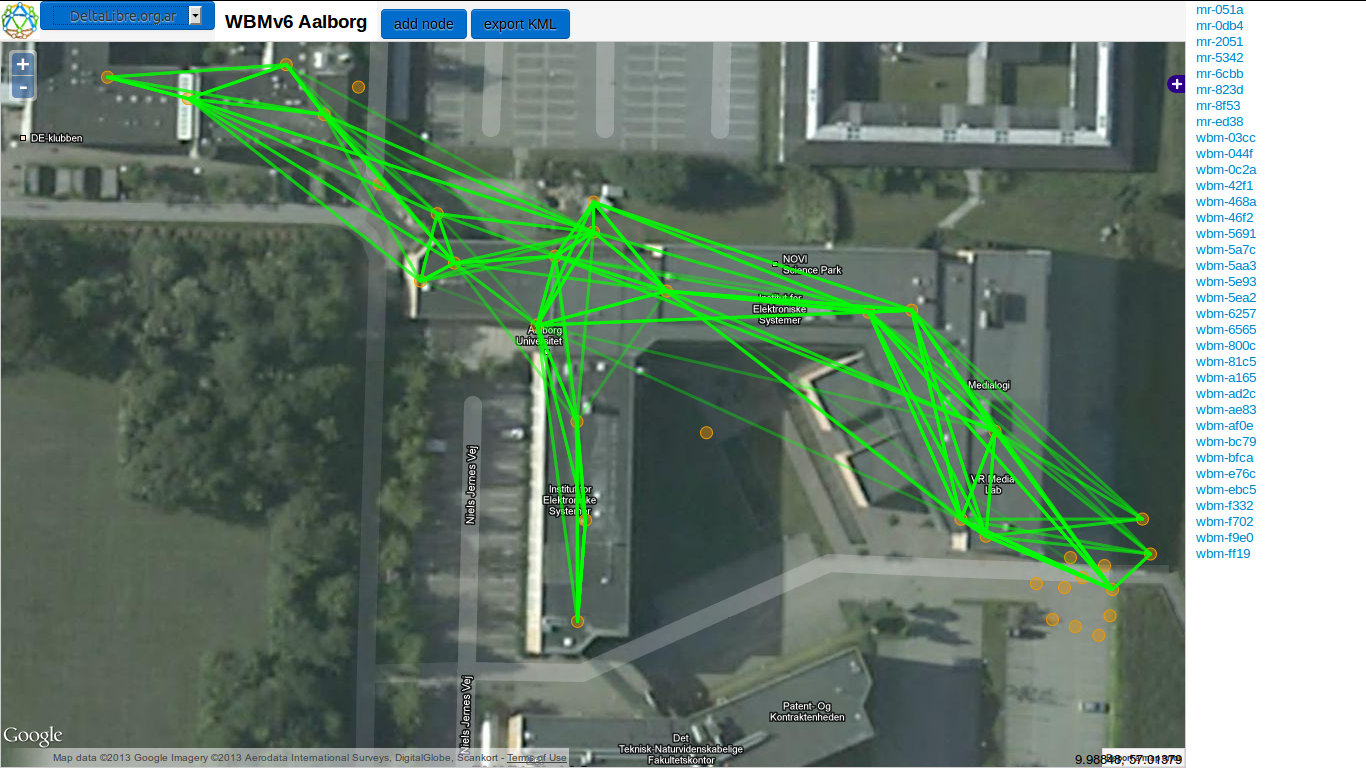
\includegraphics[width=1.4\textwidth, angle=90]{figures/geographical_map2.png}
\caption{geographical map snapshot}
\label{fig:geomap}
\end{figure}


% wget -O topo0.svg "http://battlemesh.org/BattleMeshV6/Tests?action=AttachFile&do=get&target=topo0.svg"
% \immediate\write18{ inkscape -D -z --file=topo0.svg --export-pdf=topo0.pdf }

\begin{figure}[!ht]
\centering
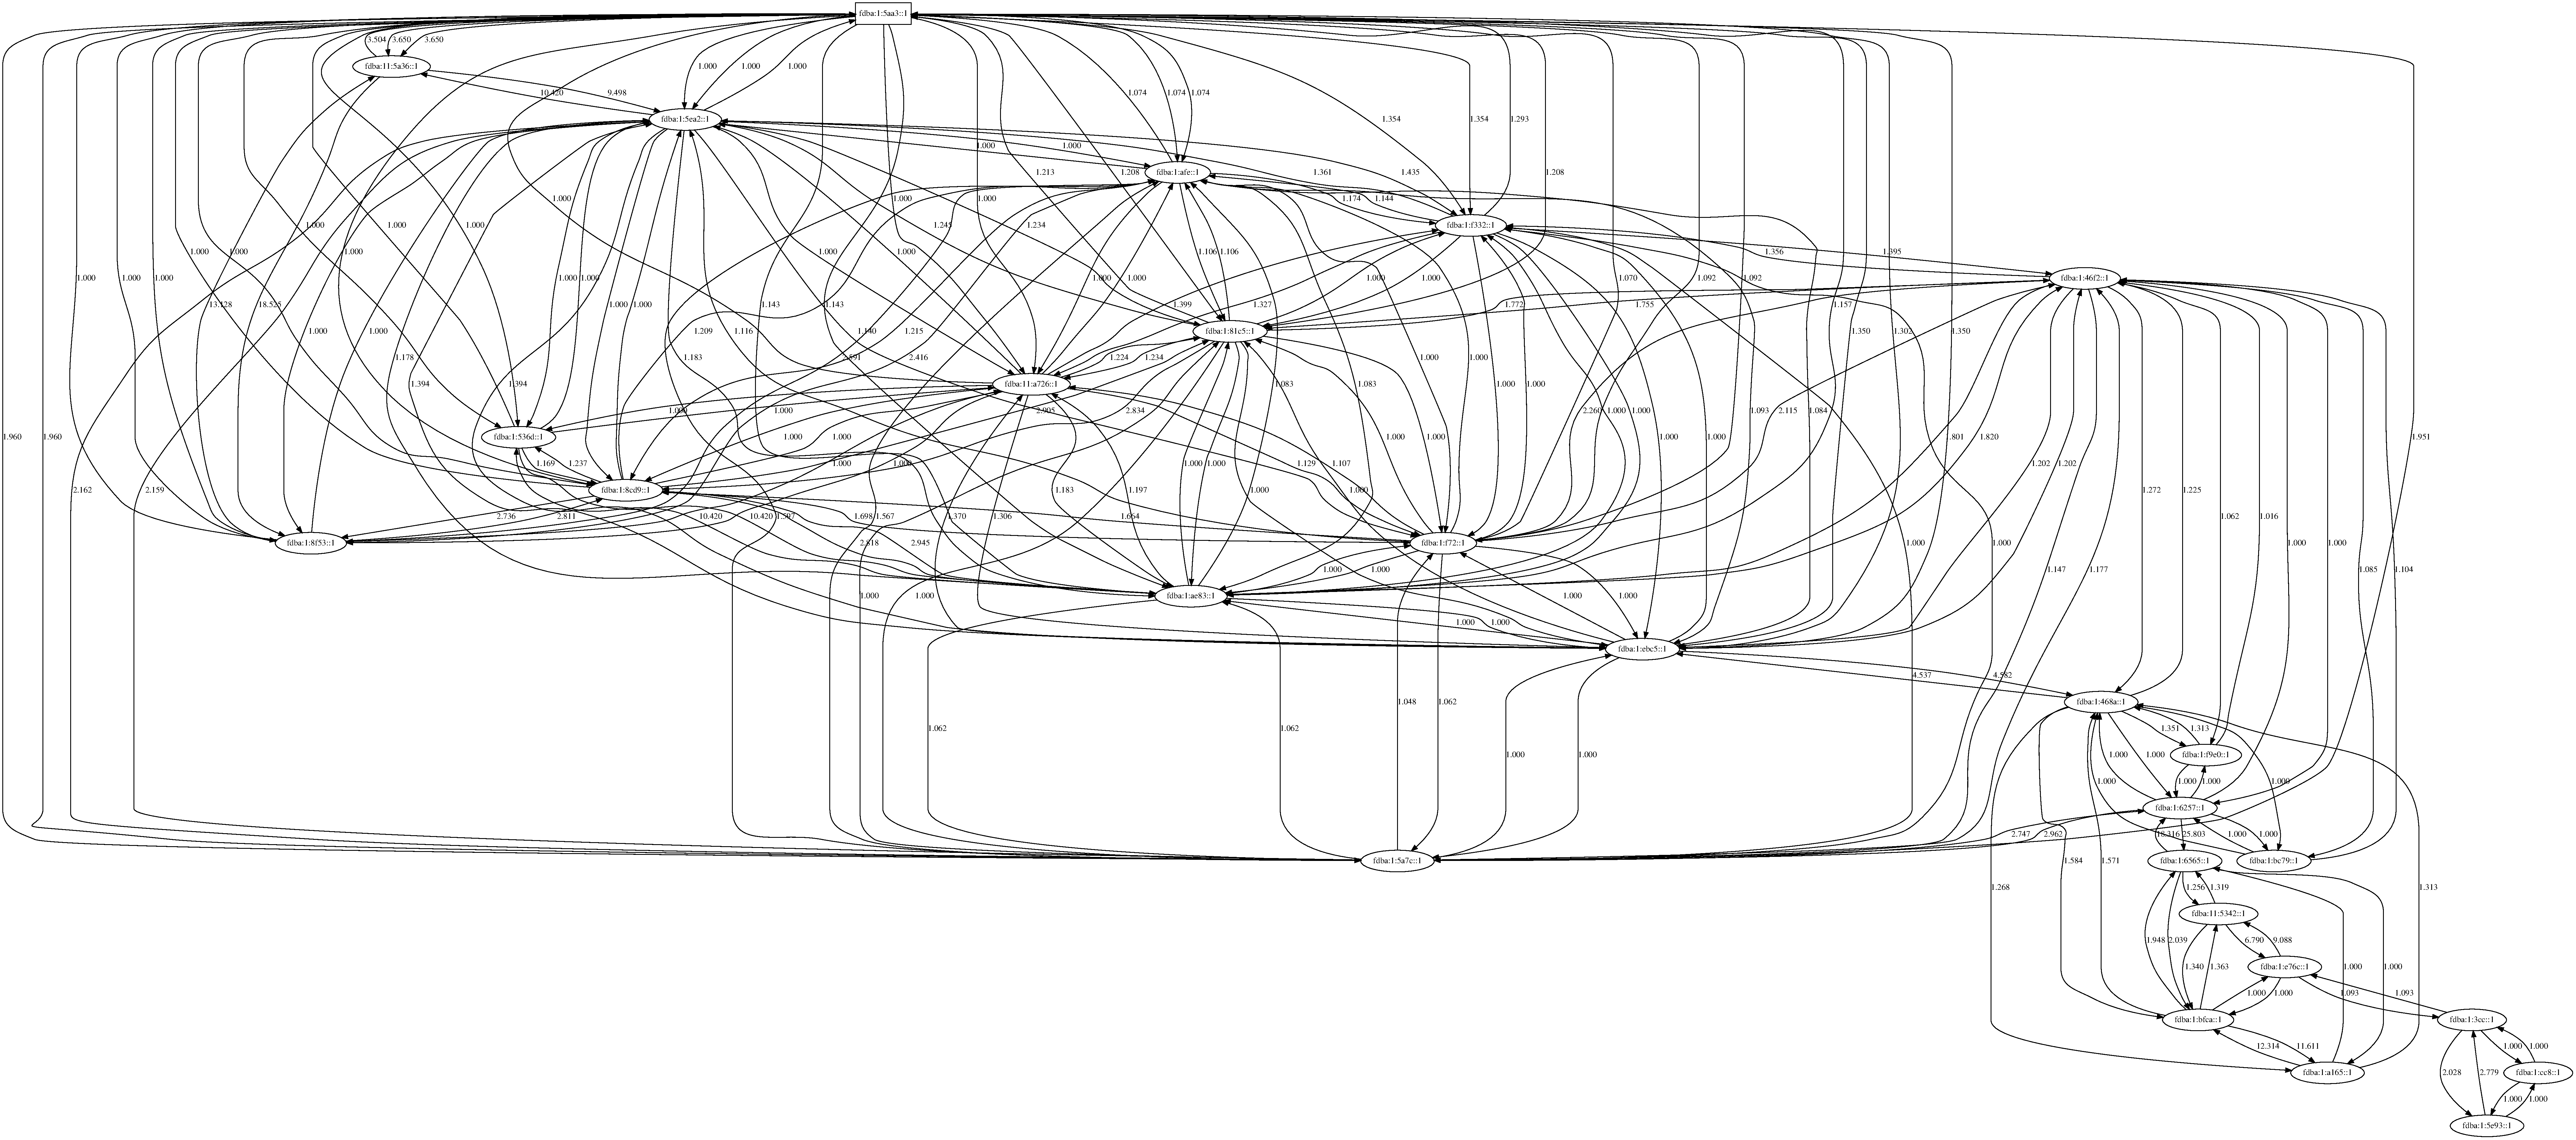
\includegraphics[width=1.4\textwidth, angle=90]{figures/topo0.pdf}
\caption{OLSR topology snapshot}
\label{fig:olsr-topo}
\end{figure}

%\begin{figure}[h]
%\centering
%\def\svgwidth{\columnwidth}
%\includesvg{topo0}
%\end{figure}

\clearpage

%%%%%%%%%%%%%%%%%%%%%%%%%%%%%%%%%%%%%%%%%%%%%%%%%%%%%%%%%%%%%%%%%%%%%%%%%%%%%%%%
%%%%%%%%%%%%%%%%%%%%%%%%%%%%%%%%%%%%%%%%%%%%%%%%%%%%%%%%%%%%%%%%%%%%%%%%%%%%%%%%
%%%%%%%%%%%%%%%%%%%%%%%%%%%%%%%%%%%%%%%%%%%%%%%%%%%%%%%%%%%%%%%%%%%%%%%%%%%%%%%%
\section{Ping Measurements (hops, rtt, loss)}
\label{sec:ping-measurements}

%%%%%%%%%%%%%%%%%%%%%%%%%%%%%%%%%%%%%%%%%%%%%%%%%%%%%%%%%%%%%%%%%%%%%%%%%%%%%%%%
\subsection{Assumptions}





%%%%%%%%%%%%%%%%%%%%%%%%%%%%%%%%%%%%%%%%%%%%%%%%%%%%%%%%%%%%%%%%%%%%%%%%%%%%%%%%
%\immediate\write18{ ../eval.R --data=../tmp.data --stat=../tmp.stat --imgdir=../img --texdir=inputs/ }

%%%%%%%%%%%%%%%%%%%%%%%%%%%%%%%%%%%%%%%%%%%%%%%%%%%%%%%%%%%%%%%%%%%%%%%%%%%%%%%%
\subsection{Stationary Scenarios}

\clearpage
\makeFigure{sArtt}{Random node test 1}{0.69}
\makeFigure{sArvh}{Random node test 1}{0.69}

\clearpage

\makeFigure{sBrtt}{Random node test 2}{0.69}
\makeFigure{sBrvh}{Random node test 2}{0.69}


\clearpage

%%%%%%%%%%%%%%%%%%%%%%%%%%%%%%%%%%%%%%%%%%%%%%%%%%%%%%%%%%%%%%%%%%%%%%%%%%%%%%%%
\subsection{Mobile Scenarios}


%\makeFigure{sArtt}{RTT ECDF of mobile and running node tests (groups 1-3)}{0.7}
%\makeFigure{sArvh}{RTT vs hops of Mobile and running node tests (groups 1-3)}{0.7}


\makeCCTabl{tbl:m0}{Mobile test 0 (group 1)} {%
      \makeTCCGraphic{m0}
}

\makeCCTabl{tbl:m1}{Mobile node test 1 (group 2)} {%
      \makeTCCGraphic{m1}
}

\makeCCTabl{tbl:m0-m2}{Running node test 2 (group 3)} {%
      \makeTCCGraphic{m2}
}



%\begin{figure}
% \centering
% \includegraphics[width=1\textwidth]{../img/out.pdf}
% \caption{Research guidelines}
% \label{fig:guidelines}
%\end{figure}


%%%%%%%%%%%%%%%%%%%%%%%%%%%%%%%%%%%%%%%%%%%%%%%%%%%%%%%%%%%%%%%%%%%%%%%%%%%%%%%%
%%%%%%%%%%%%%%%%%%%%%%%%%%%%%%%%%%%%%%%%%%%%%%%%%%%%%%%%%%%%%%%%%%%%%%%%%%%%%%%%
%%%%%%%%%%%%%%%%%%%%%%%%%%%%%%%%%%%%%%%%%%%%%%%%%%%%%%%%%%%%%%%%%%%%%%%%%%%%%%%%
\section{TCP Throughput Measurements}
\label{sec:tp-measurements}


%%%%%%%%%%%%%%%%%%%%%%%%%%%%%%%%%%%%%%%%%%%%%%%%%%%%%%%%%%%%%%%%%%%%%%%%%%%%%%%%
%%%%%%%%%%%%%%%%%%%%%%%%%%%%%%%%%%%%%%%%%%%%%%%%%%%%%%%%%%%%%%%%%%%%%%%%%%%%%%%%
%%%%%%%%%%%%%%%%%%%%%%%%%%%%%%%%%%%%%%%%%%%%%%%%%%%%%%%%%%%%%%%%%%%%%%%%%%%%%%%%
\section{Appendix}

\subsection{Ping Results Table}

The folloing verbatim table lists statistics per experiment (EXP) and group (GRP) as calculated by the lua-based
evaluation script based on the raw ping-measurements data and outputted to the file ping.stat.
Event based results are given for each received icmp response in ping.data.

% redefine \VerbatimInput
\RecustomVerbatimCommand{\VerbatimInput}{VerbatimInput}%
{fontsize=\tiny,
 %
 frame=lines,  % top and bottom rule only
 framesep=2em, % separation between frame and text
% rulecolor=\color{Gray},
 %
 label=\fbox{ping.stat},
 labelposition=topline,
 %
 commandchars=\|\(\), % escape character and argument delimiters for
                      % commands within the verbatim
 commentchar=*        % comment character
}

\VerbatimInput{../ping.stat}

\subsection{Individual Random-node Test Measurements}

\makeCCCTabl{tbl:s4-s6}{Individual Random node tests (groups 4-6)} {%
      \makeCCCGraphic{s4}
      \makeCCCGraphic{s5}
      \makeCCCGraphic{s6}
      \makeCCCGraphic{s7}
}

\makeCCCTabl{tbl:s4-s6}{Individual Random node tests (groups 8-11)} {%
      \makeCCCGraphic{s8}
      \makeCCCGraphic{s9}
      \makeCCCGraphic{s10}
      \makeCCCGraphic{s11}
}

\makeCCCTabl{tbl:s4-s6}{Individual Random node tests (groups 12-15)} {%
      \makeCCCGraphic{s12}
      \makeCCCGraphic{s13}
      \makeCCCGraphic{s14}
      \makeCCCGraphic{s15}
}

\makeCCCTabl{tbl:s4-s6}{Individual Random node tests (groups 16-19)} {%
      \makeCCCGraphic{s16}
      \makeCCCGraphic{s17}
      \makeCCCGraphic{s18}
      \makeCCCGraphic{s19}
}

\makeCCCTabl{tbl:s4-s6}{Individual Random node tests (groups 20-23)} {%
      \makeCCCGraphic{s20}
      \makeCCCGraphic{s21}
      \makeCCCGraphic{s22}
      \makeCCCGraphic{s23}
}

\makeCCCTabl{tbl:s4-s6}{Individual Random node tests (groups 24-27)} {%
      \makeCCCGraphic{s24}
      \makeCCCGraphic{s25}
      \makeCCCGraphic{s26}
      \makeCCCGraphic{s27}
}

\makeCCCTabl{tbl:s4-s6}{Individual Random node tests (groups 28-31)} {%
      \makeCCCGraphic{s28}
      \makeCCCGraphic{s29}
      \makeCCCGraphic{s30}
      \makeCCCGraphic{s31}
}

\makeCCCTabl{tbl:s4-s6}{Individual Random node tests (groups 32-35)} {%
      \makeCCCGraphic{s32}
      \makeCCCGraphic{s33}
      \makeCCCGraphic{s34}
      \makeCCCGraphic{s35}
}

\makeCCCTabl{tbl:s4-s6}{Individual Random node tests (groups 36-39)} {%
      \makeCCCGraphic{s36}
      \makeCCCGraphic{s37}
      \makeCCCGraphic{s38}
      \makeCCCGraphic{s39}
}

\makeCCCTabl{tbl:s4-s6}{Individual Random node tests (groups 40-43)} {%
      \makeCCCGraphic{s40}
      \makeCCCGraphic{s41}
      \makeCCCGraphic{s42}
      \makeCCCGraphic{s43}
}

\makeCCCTabl{tbl:s4-s6}{Individual Random node tests (groups 44-47)} {%
      \makeCCCGraphic{s44}
      \makeCCCGraphic{s45}
      \makeCCCGraphic{s46}
      \makeCCCGraphic{s47}
}

\makeCCCTabl{tbl:s4-s6}{Individual Random node tests (groups 48-50)} {%
      \makeCCCGraphic{s48}
      \makeCCCGraphic{s49}
      \makeCCCGraphic{s50}
}


%%%%%%%%%%%%%%%%%%%%%%%%%%%%%%%%%%%%%%%%%%%%%%%%%%%%%%%%%%%%%%%%%%%%%%%%%%%%%%%%
%%%%%%%%%%%%%%%%%%%%%%%%%%%%%%%%%%%%%%%%%%%%%%%%%%%%%%%%%%%%%%%%%%%%%%%%%%%%%%%%
%\section*{Acknowledgements}
%
%This work is supported by ...


%%%%%%%%%%%%%%%%%%%%%%%%%%%%%%%%%%%%%%%%%%%%%%%%%%%%%%%%%%%%%%%%%%%%%%%%%%%%%%%%
%%%%%%%%%%%%%%%%%%%%%%%%%%%%%%%%%%%%%%%%%%%%%%%%%%%%%%%%%%%%%%%%%%%%%%%%%%%%%%%%

\backmatter

\bibliographystyle{ieeetr}
%\bibliography{biblio-data}

\end{document} 
